% \VignetteIndexEntry{HelloRanges Tutorial}
% \VignetteKeywords{ranges, bedtools, tutorial}
% \VignettePackage{HelloRanges}
\documentclass[10pt]{article}

\RequirePackage[]{/Library/Frameworks/R.framework/Versions/3.3/Resources/library/BiocStyle/resources/tex/Bioconductor2}
\AtBeginDocument{\bibliographystyle{/Library/Frameworks/R.framework/Versions/3.3/Resources/library/BiocStyle/resources/tex/unsrturl}}
\usepackage[noae, nogin]{Sweave}
\bioctitle[HelloRanges Tutorial]{Saying Hello to the Bioconductor
  Ranges Infrastructure}

\author{Michael Lawrence\thanks{\email{michafla@gene.com}}\\Genentech}
\date{\today}

\usepackage{Sweave}
\begin{document}

\maketitle
\packageVersion{HelloRanges 0.0.3}
\tableofcontents
\newpage

% TODO:
% - Demonstrate visualizing some of the tracks with ggbio?

\section{Introduction}

The primary purpose of the \Biocpkg{HelloRanges} package, from the
pedagogical perspective, is to map \software{bedtools} ``recipes'' to
\R{} scripts. The package was born out of the recognition
that \Bioconductor{} lacks a cookbook that explains how to achieve
common, specific tasks using the Ranges infrastructure. And that
writing a compiler is more fun (and hopefully more useful) than
writing documentation. The goal is to enable those who already use
\R{}/\Bioconductor{} for modeling and plotting to unify their workflow
by integrating their upstream processing.

\Biocpkg{HelloRanges} provides an \R{} function corresponding to each
\software{bedtools} command. The output is an \R{} language object,
and we can print the object to copy and integrate the code into an R
script.  Ideally, the code is first integrated (by copy/paste) into an
R script. Unlike bedtools, the result of evaluation is an R object
that is suitable for further analysis. There is no automatic output to
files, because once we are in \R{}, we want to stay there. Assuming
that the reader is interested in learning Bioconductor, we encourage
the reader to inspect the code prior to evaluation by printing the
language object. The generated code is meant to be correct, readable,
conformant to best practices and performant (in that order). While the
code is much more verbose than the corresponding \software{bedtools}
call, we argue that the explicit, low-level Ranges API has the
advantage of being self-documenting and more flexible. And, of course,
it directly integrates with the rest of \Bioconductor{}.

Obviously, performing I/O with each operation will have a negative
impact on performance, so it is recommended to import the data once,
and perform subsequent operations on in-memory data structures. If
memory is exhausted, consider distributing computations.

For the sake of comparison, this tutorial closely follows that of
\software{bedtools} itself
(\url{http://quinlanlab.org/tutorials/bedtools/bedtools.html}). We
will analyze the data from Maurano et al \cite{maurano2012systematic}
assessment of DnaseI hypersensitivy across a range of fetal tissues
(20 samples). The \software{bedtools} tutorial mostly consists of
arbitrary range operations on the annotation tracks. Near the end, we
will compare samples from the Maurano study in terms of their mutual
overlap.

\section{Data}

The data are provided via the \Biocpkg{HelloRangesData} package, which
we load presently:
\begin{Schunk}
\begin{Sinput}
> library(HelloRanges)
> library(HelloRangesData)
\end{Sinput}
\end{Schunk}

To have convenient paths to the data, we switch our working directory
to the one with the data files:
\begin{Schunk}
\begin{Sinput}
> oldwd <- setwd(system.file("extdata", package="HelloRangesData"))
\end{Sinput}
\end{Schunk}

In our working directory are 20 BED files from the DnaseI study, as
well as BED files representing the CpG islands (\file{cpg.bed}),
Refseq exons (\file{exons.bed}), disease-associated SNPs
(\file{gwas.bed}), and functional annotations output by chromHMM given
ENCODE human embrionic stem cell ChIP-seq data
(\file{hesc.chromHmm.bed}). There is also a \file{hg19.genome} file
indicating the chromosome lengths of the hg19 genome build.

One of the advantages of \R{}, compared to the shell, is its unified
package management system. \R{} packages can contain data, and even
completed analyses, in addition to libraries of
functions. \Bioconductor{} provides many annotations and sample
datasets through packages. Packages make obtaining data easy, and they
also help with reproducibility and provenance through
versioning. Thus, they are more convenient and safer compared to
downloading from live URLs. Some packages provide APIs to download
data from repositories, and we can use them to programmatically
generate data packages in a reproducible way.

For example, the TxDb packages provide transcript annotations for an
individual reference genome. \Bioconductor{} provides pre-built TxDb
packages for the commonly used genome builds, and it is easy to
generate a custom TxDb package using annotations from Biomart, UCSC,
or just a GFF file. The \Biocpkg{rtracklayer} package supports
automated retrieval of any dataset from the UCSC table browser,
without any pointing-and-clicking involved. We will demonstrate some
of these tools later in the tutorial.

% Data (hg19):
% - DnaseI hypersensitivity: bedtools tutorial
% - Exons: GenomicFeatures package
% - CpG Islands: cpgIslandExt
% - Flagged SNPs: snp146Flagged
% - ChromHMM: wgEncodeBroadHmmH1hescHMM

\section{Overlap and Intersection}
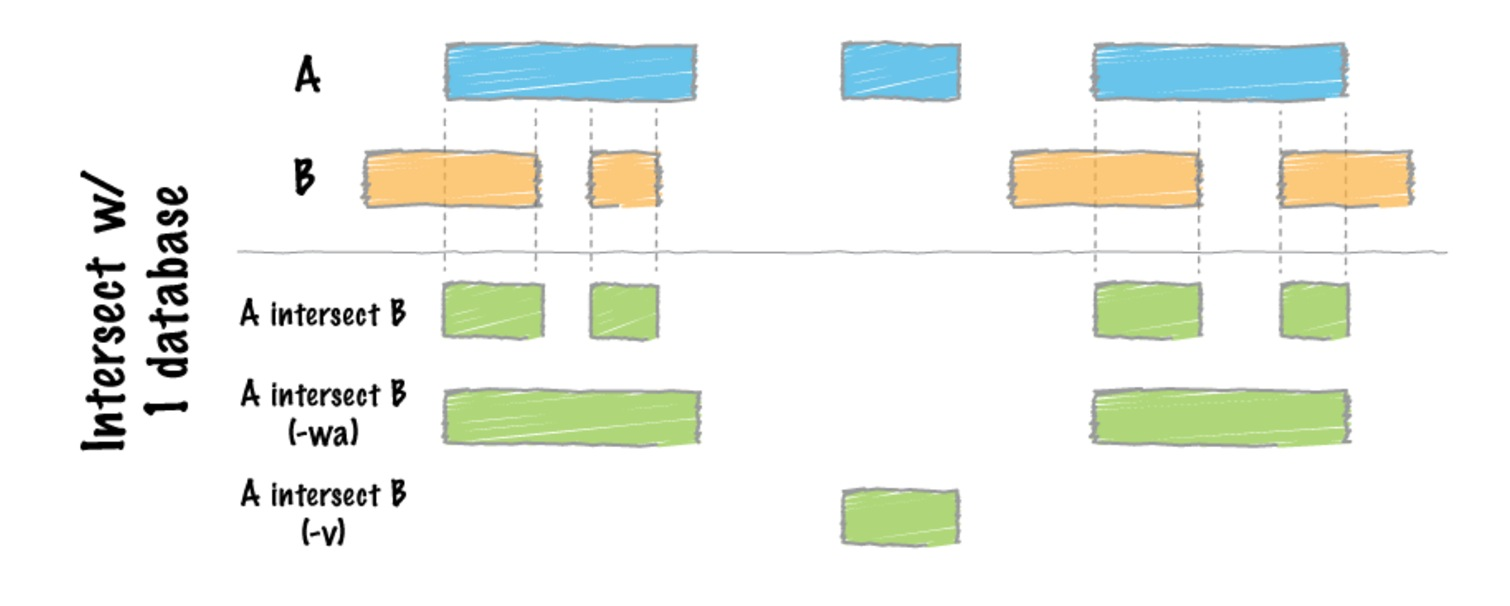
\includegraphics{fig/intersect.jpg}

One of the most useful ways to compare two tracks is to determine
which ranges overlap, and where they intersect (see the above image
from the \software{bedtools} tutorial).

By default, \software{bedtools} outputs the region of intersection for
each overlap between the two tracks. We compile the code for
intersecting the CpG islands and the exons.
\begin{Schunk}
\begin{Sinput}
> code <- bedtools_intersect("-a cpg.bed -b exons.bed -g hg19.genome")
> code
\end{Sinput}
\begin{Soutput}
{
    genome <- import("hg19.genome")
    gr_a <- import("cpg.bed", genome = genome)
    gr_b <- import("exons.bed", genome = genome)
    pairs <- findOverlapPairs(gr_a, gr_b, ignore.strand = TRUE)
    ans <- pintersect(pairs, ignore.strand = TRUE)
    ans
}
\end{Soutput}
\end{Schunk}
This code should be integrated into an R script that implements a
larger workflow. For the purposes of this tutorial, we will call
\Rfunction{eval} on the language object to yield the result:
\begin{Schunk}
\begin{Sinput}
> ans <- eval(code)
> mcols(ans)$hit <- NULL
> ans
\end{Sinput}
\begin{Soutput}
GRanges object with 45500 ranges and 1 metadata column:
          seqnames               ranges strand |        name
             <Rle>            <IRanges>  <Rle> | <character>
      [1]     chr1     [ 29321,  29370]      * |    CpG:_116
      [2]     chr1     [135125, 135563]      * |     CpG:_30
      [3]     chr1     [327791, 328229]      * |     CpG:_29
      [4]     chr1     [327791, 328229]      * |     CpG:_29
      [5]     chr1     [327791, 328229]      * |     CpG:_29
      ...      ...                  ...    ... .         ...
  [45496]     chrY [59213949, 59214117]      * |     CpG:_36
  [45497]     chrY [59213949, 59214117]      * |     CpG:_36
  [45498]     chrY [59213949, 59214117]      * |     CpG:_36
  [45499]     chrY [59213949, 59214117]      * |     CpG:_36
  [45500]     chrY [59213949, 59214117]      * |     CpG:_36
  -------
  seqinfo: 93 sequences from hg19 genome
\end{Soutput}
\end{Schunk}
%
The result is an instance of \Rclass{GRanges}, the central data
structure in \Bioconductor{} for genomic data.  A \Rclass{GRanges}
takes the form of a table and resembles a BED file, with a column for
the chromosome, start, end, strand.  We will see \Rclass{GRanges} a
lot, along with its cousin, \Rclass{GRangesList}, which stores what
\software{bedtools} calls ``split'' ranges.

\subsection{Sequence information}

Consider the simplest invocation of \software{bedtools intersect}:
\begin{Schunk}
\begin{Sinput}
> code <- bedtools_intersect("-a cpg.bed -b exons.bed")
> code
\end{Sinput}
\begin{Soutput}
{
    genome <- Seqinfo(genome = NA_character_)
    gr_a <- import("cpg.bed", genome = genome)
    gr_b <- import("exons.bed", genome = genome)
    pairs <- findOverlapPairs(gr_a, gr_b, ignore.strand = TRUE)
    ans <- pintersect(pairs, ignore.strand = TRUE)
    ans
}
\end{Soutput}
\end{Schunk}

The first line creates an object representing the structure of the
genome build:
\begin{Schunk}
\begin{Sinput}
> genome <- eval(code[[2L]])
> genome
\end{Sinput}
\begin{Soutput}
Seqinfo object with no sequences:
\end{Soutput}
\end{Schunk}
%
It is an empty object, because the genome identifier is unspecified
(\Robject{NA\_character\_}). Having unspecified genome bounds is
dangerous and leads to accidents involving incompatible genome
builds. Besides error checking, the bounds are useful when computing
coverage and finding the gaps (see below). Luckily,
\software{bedtools} lets us specify the genome as an argument:
\begin{Schunk}
\begin{Sinput}
> code <- bedtools_intersect("-a cpg.bed -b exons.bed -g hg19.genome")
> code
\end{Sinput}
\begin{Soutput}
{
    genome <- import("hg19.genome")
    gr_a <- import("cpg.bed", genome = genome)
    gr_b <- import("exons.bed", genome = genome)
    pairs <- findOverlapPairs(gr_a, gr_b, ignore.strand = TRUE)
    ans <- pintersect(pairs, ignore.strand = TRUE)
    ans
}
\end{Soutput}
\begin{Sinput}
> genome <- eval(code[[2L]])
> genome
\end{Sinput}
\begin{Soutput}
Seqinfo object with 93 sequences from hg19 genome:
  seqnames              seqlengths isCircular genome
  chr1                   249250621       <NA>   hg19
  chr10                  135534747       <NA>   hg19
  chr11                  135006516       <NA>   hg19
  chr11_gl000202_random      40103       <NA>   hg19
  chr12                  133851895       <NA>   hg19
  ...                          ...        ...    ...
  chrUn_gl000247             36422       <NA>   hg19
  chrUn_gl000248             39786       <NA>   hg19
  chrUn_gl000249             38502       <NA>   hg19
  chrX                   155270560       <NA>   hg19
  chrY                    59373566       <NA>   hg19
\end{Soutput}
\end{Schunk}
We now have a populated genome, since the tutorial had provided the
\file{hg19.genome} file. However, in general, information on the
genome build should be centralized, not sitting somewhere in a
file. \Bioconductor{} provides \Biocpkg{GenomeInfoDb} as its central
source of sequence information. We can hook into that by passing the
genome identifier instead of a file name:
\begin{Schunk}
\begin{Sinput}
> code <- bedtools_intersect("-a cpg.bed -b exons.bed -g hg19")
> genome <- eval(code[[2L]])
> genome
\end{Sinput}
\begin{Soutput}
Seqinfo object with 93 sequences (1 circular) from hg19 genome:
  seqnames       seqlengths isCircular genome
  chr1            249250621      FALSE   hg19
  chr2            243199373      FALSE   hg19
  chr3            198022430      FALSE   hg19
  chr4            191154276      FALSE   hg19
  chr5            180915260      FALSE   hg19
  ...                   ...        ...    ...
  chrUn_gl000245      36651      FALSE   hg19
  chrUn_gl000246      38154      FALSE   hg19
  chrUn_gl000247      36422      FALSE   hg19
  chrUn_gl000248      39786      FALSE   hg19
  chrUn_gl000249      38502      FALSE   hg19
\end{Soutput}
\end{Schunk}

\subsection{Annotations}

Now our code looks like:
\begin{Schunk}
\begin{Sinput}
> code
\end{Sinput}
\begin{Soutput}
{
    genome <- Seqinfo(genome = "hg19")
    gr_a <- import("cpg.bed", genome = genome)
    gr_b <- import("exons.bed", genome = genome)
    pairs <- findOverlapPairs(gr_a, gr_b, ignore.strand = TRUE)
    ans <- pintersect(pairs, ignore.strand = TRUE)
    ans
}
\end{Soutput}
\end{Schunk}
The next step is the import of the CpG islands and exons using the
\Rfunction{import} function from \Biocpkg{rtracklayer}, which can
load pretty much any kind of genomic data into the appropriate
type of \Bioconductor{} object. In this case, we are loading the data
as a \Rclass{GRanges}:
\begin{Schunk}
\begin{Sinput}
> gr_a
\end{Sinput}
\begin{Soutput}
GRanges object with 28691 ranges and 1 metadata column:
          seqnames               ranges strand |        name
             <Rle>            <IRanges>  <Rle> | <character>
      [1]     chr1     [ 28736,  29810]      * |    CpG:_116
      [2]     chr1     [135125, 135563]      * |     CpG:_30
      [3]     chr1     [327791, 328229]      * |     CpG:_29
      [4]     chr1     [437152, 438164]      * |     CpG:_84
      [5]     chr1     [449274, 450544]      * |     CpG:_99
      ...      ...                  ...    ... .         ...
  [28687]     chrY [27610116, 27611088]      * |     CpG:_76
  [28688]     chrY [28555536, 28555932]      * |     CpG:_32
  [28689]     chrY [28773316, 28773544]      * |     CpG:_25
  [28690]     chrY [59213795, 59214183]      * |     CpG:_36
  [28691]     chrY [59349267, 59349574]      * |     CpG:_29
  -------
  seqinfo: 93 sequences from hg19 genome
\end{Soutput}
\end{Schunk}

The \Biocpkg{rtracklayer} package can also download data directly from
the UCSC table browser. For example, we could get the CpG islands directly:
\begin{Schunk}
\begin{Sinput}
> ucsc <- browserSession()
> genome(ucsc) <- "hg19"
> cpgs <- ucsc[["CpG Islands"]]
\end{Sinput}
\end{Schunk}

Gene annotations, including exon coordinates, should also be stored
more formally than in a file, and Bioconductor provides them through
its TxDb family of packages:
\begin{Schunk}
\begin{Sinput}
> library(TxDb.Hsapiens.UCSC.hg19.knownGene)
> exons <- exons(TxDb.Hsapiens.UCSC.hg19.knownGene)
\end{Sinput}
\end{Schunk}

\subsection{Finding Overlaps}

A review of the code:
\begin{Schunk}
\begin{Sinput}
> code
\end{Sinput}
\begin{Soutput}
{
    genome <- Seqinfo(genome = "hg19")
    gr_a <- import("cpg.bed", genome = genome)
    gr_b <- import("exons.bed", genome = genome)
    pairs <- findOverlapPairs(gr_a, gr_b, ignore.strand = TRUE)
    ans <- pintersect(pairs, ignore.strand = TRUE)
    ans
}
\end{Soutput}
\end{Schunk}

The next step is to find all of the overlaps. The workhorse function
is \Rfunction{findOverlaps} from the \Biocpkg{IRanges} package. Here,
we use the variant \Rfunction{findOverlapPairs}, a convenience for
creating a \Rclass{Pairs} object that matches up the overlapping
ranges:
\begin{Schunk}
\begin{Sinput}
> pairs
\end{Sinput}
\begin{Soutput}
Pairs object with 45500 pairs and 0 metadata columns:
                           first                   second
                       <GRanges>                <GRanges>
      [1]       chr1:28736-29810       chr1:29321-29370:-
      [2]     chr1:135125-135563     chr1:134773-139696:-
      [3]     chr1:327791-328229     chr1:324439-328581:+
      [4]     chr1:327791-328229     chr1:324439-328581:+
      [5]     chr1:327791-328229     chr1:327036-328581:+
      ...                    ...                      ...
  [45496] chrY:59213795-59214183 chrY:59213949-59214117:+
  [45497] chrY:59213795-59214183 chrY:59213949-59214117:+
  [45498] chrY:59213795-59214183 chrY:59213949-59214117:+
  [45499] chrY:59213795-59214183 chrY:59213949-59214117:+
  [45500] chrY:59213795-59214183 chrY:59213949-59214117:+
\end{Soutput}
\end{Schunk}
Although the ranges are displayed as succinct strings, they data are
still represented as \Rclass{GRanges} objects.

Users of \software{bedtools} will be familiar with \Rclass{Pairs} as
the analog of the BEDPE file format. We can use \Biocpkg{rtracklayer}
to export \Rclass{Pairs} to BEDPE:
\begin{Schunk}
\begin{Sinput}
> export(pairs, "pairs.bedpe")
\end{Sinput}
\end{Schunk}

A key parameter to \Rfunction{findOverlapPairs} is
\Rcode{ignore.strand=TRUE}. By default, all operations on
\Rclass{GRanges} take strand into account when determining whether two
ranges overlap, and deciding on the orientation of a range. This is
surprising to many novice users, particularly to those with
\software{bedtools} experience. Most functions take the
\Robject{ignore.strand} argument to control this behavior. To avoid
confusion, the code generated by \Biocpkg{HelloRanges} is always
explicit about how it is treating strand. Users are encouraged to
follow the same practice.

\subsection{Computing intersections}
One last look at the code:
\begin{Schunk}
\begin{Sinput}
> code
\end{Sinput}
\begin{Soutput}
{
    genome <- Seqinfo(genome = "hg19")
    gr_a <- import("cpg.bed", genome = genome)
    gr_b <- import("exons.bed", genome = genome)
    pairs <- findOverlapPairs(gr_a, gr_b, ignore.strand = TRUE)
    ans <- pintersect(pairs, ignore.strand = TRUE)
    ans
}
\end{Soutput}
\end{Schunk}

The final step is to find the actual intersecting region between the
member of each overlapping pair. We do this with the
\Rfunction{pintersect} function, which is the ``parallel'' or
``pairwise'' version of the default \Rfunction{intersect} function. If
we had just called \Rcode{intersect(gr\_a, gr\_b)} instead, the entire
set of ranges would have been treated as a set, and overlapping ranges
in \Robject{gr\_a} and \Robject{gr\_b} would have been merged (this is
rarely desirable and requires an extra merge step in
\software{bedtools}).

Notice again the importance of \Rcode{ignore.strand=TRUE}. Without
that, ranges on opposite strands would have zero intersection.

And here is our result:
\begin{Schunk}
\begin{Sinput}
> ans
\end{Sinput}
\begin{Soutput}
GRanges object with 45500 ranges and 1 metadata column:
          seqnames               ranges strand |        name
             <Rle>            <IRanges>  <Rle> | <character>
      [1]     chr1     [ 29321,  29370]      * |    CpG:_116
      [2]     chr1     [135125, 135563]      * |     CpG:_30
      [3]     chr1     [327791, 328229]      * |     CpG:_29
      [4]     chr1     [327791, 328229]      * |     CpG:_29
      [5]     chr1     [327791, 328229]      * |     CpG:_29
      ...      ...                  ...    ... .         ...
  [45496]     chrY [59213949, 59214117]      * |     CpG:_36
  [45497]     chrY [59213949, 59214117]      * |     CpG:_36
  [45498]     chrY [59213949, 59214117]      * |     CpG:_36
  [45499]     chrY [59213949, 59214117]      * |     CpG:_36
  [45500]     chrY [59213949, 59214117]      * |     CpG:_36
  -------
  seqinfo: 93 sequences from hg19 genome
\end{Soutput}
\end{Schunk}
Again, a \Rclass{GRanges} object. The \Robject{hit} column indicates
whether the pair overlapped at all (as opposed to one range being of
zero width). It's useless in this case.

\subsection{Keeping the original features}

To keep the original form of the overlapping features, the generated
code simply neglect to call \Rfunction{pintersect} and end up with the
\Robject{pairs} object introduced previously:
\begin{Schunk}
\begin{Sinput}
> code <- bedtools_intersect("-a cpg.bed -b exons.bed -g hg19 -wa -wb")
> code
\end{Sinput}
\begin{Soutput}
{
    genome <- Seqinfo(genome = "hg19")
    gr_a <- import("cpg.bed", genome = genome)
    gr_b <- import("exons.bed", genome = genome)
    pairs <- findOverlapPairs(gr_a, gr_b, ignore.strand = TRUE)
    ans <- pairs
    ans
}
\end{Soutput}
\begin{Sinput}
> eval(code)
\end{Sinput}
\begin{Soutput}
Pairs object with 45500 pairs and 0 metadata columns:
                           first                   second
                       <GRanges>                <GRanges>
      [1]       chr1:28736-29810       chr1:29321-29370:-
      [2]     chr1:135125-135563     chr1:134773-139696:-
      [3]     chr1:327791-328229     chr1:324439-328581:+
      [4]     chr1:327791-328229     chr1:324439-328581:+
      [5]     chr1:327791-328229     chr1:327036-328581:+
      ...                    ...                      ...
  [45496] chrY:59213795-59214183 chrY:59213949-59214117:+
  [45497] chrY:59213795-59214183 chrY:59213949-59214117:+
  [45498] chrY:59213795-59214183 chrY:59213949-59214117:+
  [45499] chrY:59213795-59214183 chrY:59213949-59214117:+
  [45500] chrY:59213795-59214183 chrY:59213949-59214117:+
\end{Soutput}
\end{Schunk}

\subsection{Computing the amount of overlap}

To compute the width of the overlapping regions, we query the initial
result for its width and store as an annotation on the pairs:
\begin{Schunk}
\begin{Sinput}
> code <- bedtools_intersect("-a cpg.bed -b exons.bed -g hg19 -wo")
> code
\end{Sinput}
\begin{Soutput}
{
    genome <- Seqinfo(genome = "hg19")
    gr_a <- import("cpg.bed", genome = genome)
    gr_b <- import("exons.bed", genome = genome)
    pairs <- findOverlapPairs(gr_a, gr_b, ignore.strand = TRUE)
    ans <- pairs
    mcols(ans)$overlap_width <- width(pintersect(ans, ignore.strand = TRUE))
    ans
}
\end{Soutput}
\begin{Sinput}
> eval(code)
\end{Sinput}
\begin{Soutput}
Pairs object with 45500 pairs and 1 metadata column:
                           first                   second |
                       <GRanges>                <GRanges> |
      [1]       chr1:28736-29810       chr1:29321-29370:- |
      [2]     chr1:135125-135563     chr1:134773-139696:- |
      [3]     chr1:327791-328229     chr1:324439-328581:+ |
      [4]     chr1:327791-328229     chr1:324439-328581:+ |
      [5]     chr1:327791-328229     chr1:327036-328581:+ |
      ...                    ...                      ... .
  [45496] chrY:59213795-59214183 chrY:59213949-59214117:+ |
  [45497] chrY:59213795-59214183 chrY:59213949-59214117:+ |
  [45498] chrY:59213795-59214183 chrY:59213949-59214117:+ |
  [45499] chrY:59213795-59214183 chrY:59213949-59214117:+ |
  [45500] chrY:59213795-59214183 chrY:59213949-59214117:+ |
          overlap_width
              <integer>
      [1]            50
      [2]           439
      [3]           439
      [4]           439
      [5]           439
      ...           ...
  [45496]           169
  [45497]           169
  [45498]           169
  [45499]           169
  [45500]           169
\end{Soutput}
\end{Schunk}

This code reveals that \Rclass{GRanges}, along with every other
vector-like object in the Ranges infrastructure, is capable of storing
tabular annotations, accessible via \Rfunction{mcols}. We actually saw
this before with the ``name'' column on the Cpg Islands. Here, we use
it to store the overlap width.

\subsection{Counting the number of overlaps}

A common query, particularly in RNA-seq analysis, is how many ranges
in the subject overlap each query range. The \Rfunction{countOverlaps}
function serves this particular purpose:
\begin{Schunk}
\begin{Sinput}
> code <- bedtools_intersect("-a cpg.bed -b exons.bed -g hg19 -c")
> code
\end{Sinput}
\begin{Soutput}
{
    genome <- Seqinfo(genome = "hg19")
    gr_a <- import("cpg.bed", genome = genome)
    gr_b <- import("exons.bed", genome = genome)
    ans <- gr_a
    mcols(ans)$overlap_count <- countOverlaps(gr_a, gr_b, ignore.strand = TRUE)
    ans
}
\end{Soutput}
\begin{Sinput}
> eval(code)
\end{Sinput}
\begin{Soutput}
GRanges object with 28691 ranges and 2 metadata columns:
          seqnames               ranges strand |        name
             <Rle>            <IRanges>  <Rle> | <character>
      [1]     chr1     [ 28736,  29810]      * |    CpG:_116
      [2]     chr1     [135125, 135563]      * |     CpG:_30
      [3]     chr1     [327791, 328229]      * |     CpG:_29
      [4]     chr1     [437152, 438164]      * |     CpG:_84
      [5]     chr1     [449274, 450544]      * |     CpG:_99
      ...      ...                  ...    ... .         ...
  [28687]     chrY [27610116, 27611088]      * |     CpG:_76
  [28688]     chrY [28555536, 28555932]      * |     CpG:_32
  [28689]     chrY [28773316, 28773544]      * |     CpG:_25
  [28690]     chrY [59213795, 59214183]      * |     CpG:_36
  [28691]     chrY [59349267, 59349574]      * |     CpG:_29
          overlap_count
              <integer>
      [1]             1
      [2]             1
      [3]             3
      [4]             0
      [5]             0
      ...           ...
  [28687]             0
  [28688]             0
  [28689]             0
  [28690]             5
  [28691]             0
  -------
  seqinfo: 93 sequences (1 circular) from hg19 genome
\end{Soutput}
\end{Schunk}

\subsection{Excluding queries with overlaps}

We might instead want to exclude all query ranges that overlap any
subject range, i.e., any CpG island that overlaps an exon. The
\Rfunction{subsetByOverlaps} function is tasked with restricting by
overlap. By passing \Rcode{invert=TRUE}, we exclude ranges with
overlaps.
\begin{Schunk}
\begin{Sinput}
> code <- bedtools_intersect("-a cpg.bed -b exons.bed -g hg19 -v")
> code
\end{Sinput}
\begin{Soutput}
{
    genome <- Seqinfo(genome = "hg19")
    gr_a <- import("cpg.bed", genome = genome)
    gr_b <- import("exons.bed", genome = genome)
    subsetByOverlaps(gr_a, gr_b, invert = TRUE, ignore.strand = TRUE)
}
\end{Soutput}
\end{Schunk}

\subsection{Restricting by fraction of overlap}

The \software{bedtools} suite has deep support for restricting
overlaps by the fraction of the query/subject range that is
overlapped. This is not directly supported by the \Bioconductor{}
infrastructure, but we can filter post-hoc:
\begin{Schunk}
\begin{Sinput}
> code <- bedtools_intersect("-a cpg.bed -b exons.bed -g hg19 -f 0.5 -wo")
> code
\end{Sinput}
\begin{Soutput}
{
    genome <- Seqinfo(genome = "hg19")
    gr_a <- import("cpg.bed", genome = genome)
    gr_b <- import("exons.bed", genome = genome)
    pairs <- findOverlapPairs(gr_a, gr_b, ignore.strand = TRUE)
    olap <- pintersect(pairs, ignore.strand = TRUE)
    keep <- width(olap)/width(first(pairs)) >= 0.5
    pairs <- pairs[keep]
    ans <- pairs
    mcols(ans)$overlap_width <- width(olap)[keep]
    ans
}
\end{Soutput}
\end{Schunk}

\subsection{Performance}

Comparing the performance of \software{bedtools} and \Biocpkg{IRanges}
is like comparing apples and oranges. The typical \Bioconductor{}
workflow imports the data once, paying an upfront cost, and then
operates efficiently on in-memory data structures. The BED parser is
implemented in R code and will not compete with the parsing
performance of special purpose C code. The intersect operation itself
is also slower than \software{bedtools}, but it's still reasonably
close for being mostly implemented in R.
\begin{Schunk}
\begin{Sinput}
> a <- import("exons.bed")
> b <- import("hesc.chromHmm.bed")
> system.time(pintersect(findOverlapPairs(a, b, ignore.strand=TRUE),
+                        ignore.strand=TRUE))
\end{Sinput}
\begin{Soutput}
   user  system elapsed 
  0.540   0.069   0.610 
\end{Soutput}
\end{Schunk}

\subsection{Multiple subjects}

Often, we are interested in intersections with mutiple annotation
tracks, or multiple samples. Note that the command line parser used by
\Biocpkg{helloRanges} requires that the filenames be comma-separated,
instead of space-separated. This is probably more readable anyway.
\begin{Schunk}
\begin{Sinput}
> code <- bedtools_intersect(
+     paste("-a exons.bed",
+           "-b cpg.bed,gwas.bed,hesc.chromHmm.bed -wa -wb -g hg19",
+           "-names cpg,gwas,chromhmm"))
> ans <- eval(code)
> code
\end{Sinput}
\begin{Soutput}
{
    genome <- Seqinfo(genome = "hg19")
    gr_a <- import("exons.bed", genome = genome)
    b <- c("cpg.bed", "gwas.bed", "hesc.chromHmm.bed")
    names(b) <- c("cpg", "gwas", "chromhmm")
    bl <- List(lapply(b, import, genome = genome))
    gr_b <- stack(bl, "b")
    pairs <- findOverlapPairs(gr_a, gr_b, ignore.strand = TRUE)
    ans <- pairs
    ans
}
\end{Soutput}
\end{Schunk}
Inspecting the code, we see that we need to loop over the database
files and then \Rfunction{stack} them into a single \Rclass{GRanges}
grouped by the column ``b'':
\begin{Schunk}
\begin{Sinput}
> second(ans)
\end{Sinput}
\begin{Soutput}
GRanges object with 541205 ranges and 2 metadata columns:
           seqnames               ranges strand |        b
              <Rle>            <IRanges>  <Rle> |    <Rle>
       [1]     chr1       [11538, 11937]      * | chromhmm
       [2]     chr1       [11938, 12137]      * | chromhmm
       [3]     chr1       [12138, 14137]      * | chromhmm
       [4]     chr1       [12138, 14137]      * | chromhmm
       [5]     chr1       [12138, 14137]      * | chromhmm
       ...      ...                  ...    ... .      ...
  [541201]     chrY [59213795, 59214183]      * |      cpg
  [541202]     chrY [59213795, 59214183]      * |      cpg
  [541203]     chrY [59213795, 59214183]      * |      cpg
  [541204]     chrY [59213795, 59214183]      * |      cpg
  [541205]     chrY [59213795, 59214183]      * |      cpg
                        name
                 <character>
       [1]       11_Weak_Txn
       [2] 14_Repetitive/CNV
       [3]       11_Weak_Txn
       [4]       11_Weak_Txn
       [5]       11_Weak_Txn
       ...               ...
  [541201]           CpG:_36
  [541202]           CpG:_36
  [541203]           CpG:_36
  [541204]           CpG:_36
  [541205]           CpG:_36
  -------
  seqinfo: 93 sequences (1 circular) from hg19 genome
\end{Soutput}
\end{Schunk}
The ``b'' column is an \Rclass{Rle} object, a run-length encoded form
of an ordinary R vector, in this case a factor.  Since the data are
sorted into groups, this encoding is more efficient than a dense
representation. The ``seqnames'' and ``strand'' columns also benefit
from run-length encoding. Not only can we fit more data into memory,
many operations become faster.

\section{Merge}
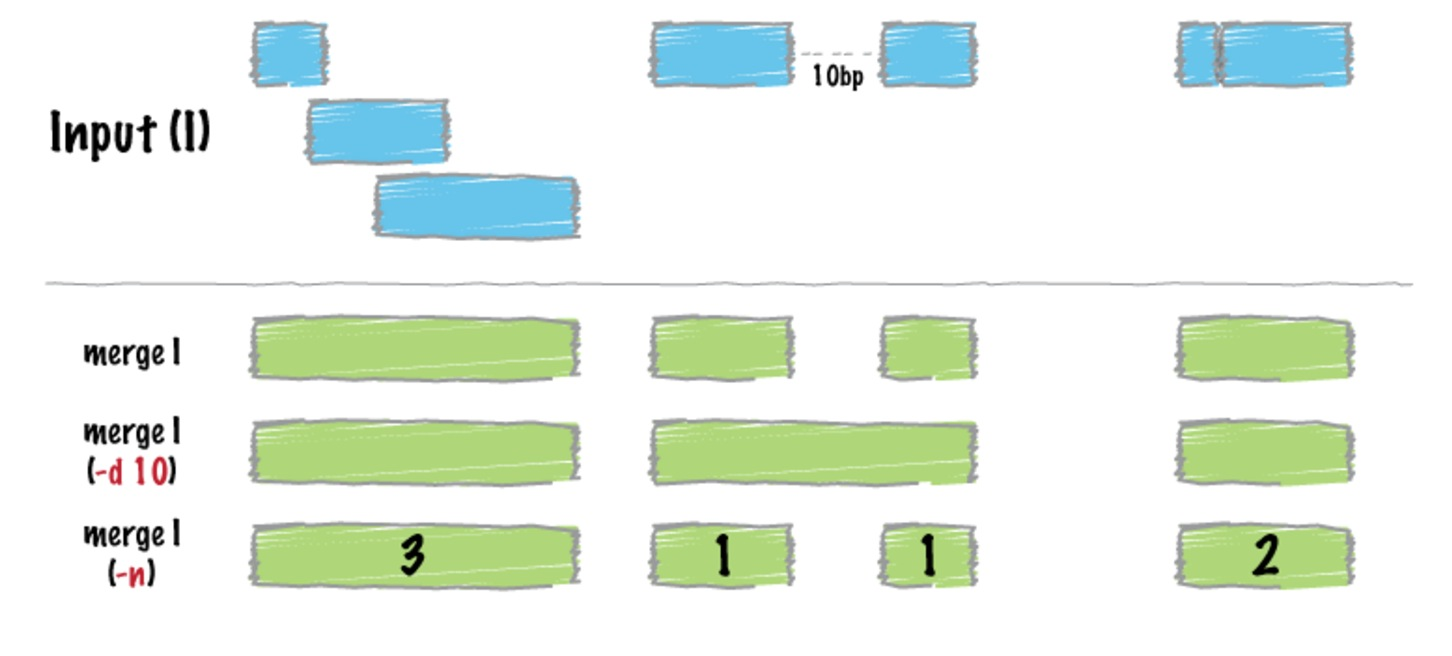
\includegraphics{fig/merge.jpg}

There are many ways to summarize interval data. In the Ranges
infrastructure, we call some of them \Rfunction{range} (min start to
max end), \Rfunction{reduce} (\software{bedtools merge}),
\Rfunction{disjoin} (involved in \software{bedtools multiinter}) and
\Rfunction{coverage} (counting the number of ranges overlapping each
position, \software{bedtools genomecov}). We are presently concerned
with \Rfunction{reduce}, which combines overlapping and adjacent
ranges into a single range. The corresponding \software{bedtools
  merge} command requires the data to be sorted; however,
\Rfunction{reduce} does not have this constraint.

\begin{Schunk}
\begin{Sinput}
> code <- bedtools_merge("-i exons.bed")
> code
\end{Sinput}
\begin{Soutput}
{
    genome <- Seqinfo(genome = NA_character_)
    gr_a <- import("exons.bed", genome = genome)
    ans <- reduce(gr_a, ignore.strand = TRUE)
    ans
}
\end{Soutput}
\end{Schunk}

\subsection{Aggregation}

As with any reduction, we often want to simultaneously aggregate
associated variables and report the summaries in the result.

We count the number of ranges overlapping each merged range:
\begin{Schunk}
\begin{Sinput}
> code <- bedtools_merge("-i exons.bed -c 1 -o count")
> code
\end{Sinput}
\begin{Soutput}
{
    genome <- Seqinfo(genome = NA_character_)
    gr_a <- import("exons.bed", genome = genome)
    ans <- reduce(gr_a, ignore.strand = TRUE, with.revmap = TRUE)
    mcols(ans) <- aggregate(gr_a, mcols(ans)$revmap, seqnames.count = lengths(seqnames), 
        drop = FALSE)
    ans
}
\end{Soutput}
\end{Schunk}

The key to aggregation with \Rfunction{reduce} is the
\Rcode{with.revmap=TRUE} argument. That yields a ``revmap'' column on
the result. It is an \Rclass{IntegerList} holding the subscripts
corresponding to each group. We pass it to \Rfunction{aggregate} to
indicate the grouping. The named arguments to \Rfunction{aggregate},
in this case \Robject{seqnames.count}, are effectively evaluated with
respect to each group (although they are actually evaluated only once).

This yields the result:
\begin{Schunk}
\begin{Sinput}
> eval(code)
\end{Sinput}
\begin{Soutput}
GRanges object with 229241 ranges and 2 metadata columns:
           seqnames               ranges strand |
              <Rle>            <IRanges>  <Rle> |
       [1]     chr1       [11874, 12227]      * |
       [2]     chr1       [12613, 12721]      * |
       [3]     chr1       [13221, 14829]      * |
       [4]     chr1       [14970, 15038]      * |
       [5]     chr1       [15796, 15947]      * |
       ...      ...                  ...    ... .
  [229237]     chrY [59337091, 59337236]      * |
  [229238]     chrY [59337949, 59338150]      * |
  [229239]     chrY [59338754, 59338859]      * |
  [229240]     chrY [59340194, 59340278]      * |
  [229241]     chrY [59342487, 59343488]      * |
                       grouping seqnames.count
           <ManyToManyGrouping>      <integer>
       [1]                    1              1
       [2]                    2              1
       [3]                  3,4              2
       [4]                    5              1
       [5]                    6              1
       ...                  ...            ...
  [229237]        459744,459745              2
  [229238]        459746,459747              2
  [229239]        459748,459749              2
  [229240]               459750              1
  [229241]        459751,459752              2
  -------
  seqinfo: 49 sequences from an unspecified genome; no seqlengths
\end{Soutput}
\end{Schunk}
We see that the grouping has been preserved on the object, in case we
wish to aggregate further through joins.

Counting the overlaps by counting the ``seqnames'' is a little
circuitous. Instead, we could have just counted the elements in each group:
\begin{Schunk}
\begin{Sinput}
> identical(lengths(ans$grouping), ans$seqnames.count)
\end{Sinput}
\begin{Soutput}
[1] TRUE
\end{Soutput}
\end{Schunk}
Note that this counting is very fast, because the ``revmap''
\Rclass{IntegerList} is not actually a list, but a partitioned vector,
and the partitioning already encodes the counts. This is an example of
where the flexibility and efficient in-memory representations of
\Bioconductor{} are particularly effective.

\subsection{Merging close features}

By default, features are merged if they are overlapping or adjacent,
i.e., the \Robject{min.gapwidth} (the minimum gap allowed to not be
merged) is 1. To merge features that are up to, say, 1000bp away, we
need to pass \Rcode{min.gapwidth=1001}:
\begin{Schunk}
\begin{Sinput}
> code <- bedtools_merge("-i exons.bed -d 1000")
> code
\end{Sinput}
\begin{Soutput}
{
    genome <- Seqinfo(genome = NA_character_)
    gr_a <- import("exons.bed", genome = genome)
    ans <- reduce(gr_a, ignore.strand = TRUE, min.gapwidth = 1001L)
    ans
}
\end{Soutput}
\end{Schunk}

Here is another example showing how to merge multiple columns at once:
\begin{Schunk}
\begin{Sinput}
> code <- bedtools_merge("-i exons.bed -d 90 -c 1,4 -o count,collapse")
> code
\end{Sinput}
\begin{Soutput}
{
    genome <- Seqinfo(genome = NA_character_)
    gr_a <- import("exons.bed", genome = genome)
    ans <- reduce(gr_a, ignore.strand = TRUE, with.revmap = TRUE, 
        min.gapwidth = 91L)
    mcols(ans) <- aggregate(gr_a, mcols(ans)$revmap, seqnames.count = lengths(seqnames), 
        name.collapse = unstrsplit(name, ","), drop = FALSE)
    ans
}
\end{Soutput}
\end{Schunk}

\section{Finding the Gaps}
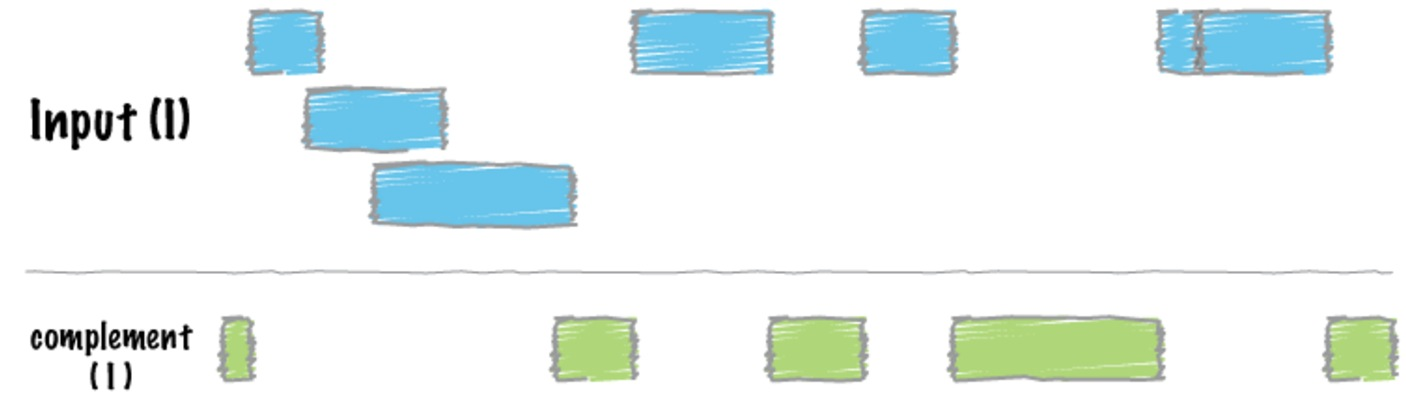
\includegraphics{fig/complement.jpg}

The \software{bedtools complement} tool finds the gaps in the
sequence, i.e., the regions of sequence the track does not cover. This
is where having the sequence bounds is critical.

\begin{Schunk}
\begin{Sinput}
> code <- bedtools_complement("-i exons.bed -g hg19.genome")
> code
\end{Sinput}
\begin{Soutput}
{
    genome <- import("hg19.genome")
    gr_a <- import("exons.bed", genome = genome)
    ans <- setdiff(as(seqinfo(gr_a), "GRanges"), unstrand(gr_a))
    ans
}
\end{Soutput}
\end{Schunk}

The call to \Rfunction{setdiff} is a set operation, along with
\Rfunction{intersect} and \Rfunction{union}. Set operations behave a
bit surprisingly with respect to strand. The ``unstranded'' features,
those with ``*'' for their strand, are considered to be in a separate
space from the stranded features. If we pass
\Rcode{ignore.strand=TRUE}, both arguments are unstranded and the
result is unstranded (strand information is discarded). This makes
sense, because there is no obvious way to merge a stranded and
unstranded feature. Since we are looking for the gaps, we do not care
about the strand, so discarding the strand is acceptable. Best
practice is to make this explicit by calling \Rfunction{unstrand}
instead of assuming the reader understands the behavior of
\Rcode{ignore.strand=TRUE}.

\section{Computing Genomic Coverage}
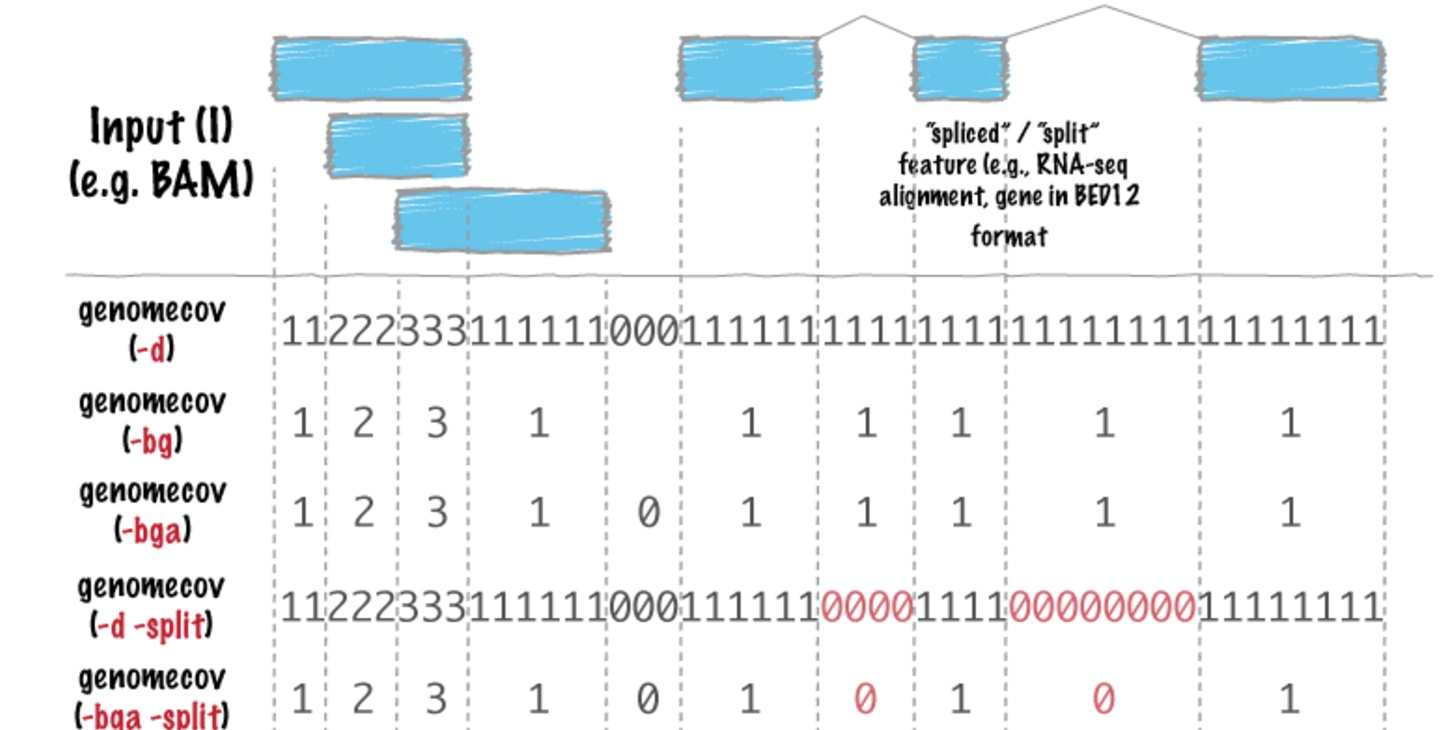
\includegraphics{fig/genomecov.jpg}

One of the useful ways to summarize ranges, particularly alignments,
is to count how many times a position is overlapped by a range. This
is called the coverage. Unlike \software{bedtools genomecov}, we do
not require the data to be sorted.

\subsection{Coverage vector}

To compute the coverage, we just call \Rfunction{coverage}. For
consistency with \software{bedtools}, which drops zero runs with the
``-bg'' option, we convert the coverage vector to a \Rclass{GRanges}
and subset:
\begin{Schunk}
\begin{Sinput}
> code <- bedtools_genomecov("-i exons.bed -g hg19.genome -bg")
> code
\end{Sinput}
\begin{Soutput}
{
    genome <- import("hg19.genome")
    gr_a <- import("exons.bed", genome = genome)
    cov <- coverage(gr_a)
    ans <- GRanges(cov)
    ans <- subset(ans, score > 0)
    ans
}
\end{Soutput}
\end{Schunk}

\subsection{Coverage histogram}

The default behavior of \software{genomecov} is to compute a histogram
showing the number and fraction of positions covered at each level. It
does this for the individual chromosome, and the entire genome. While
computing the coverage vector is as simple as calling
\Rfunction{coverage}, forming the histogram is a bit
complicated. This is a bit esoteric, but it lets us
demonstrate how to aggregate data in R:
\begin{Schunk}
\begin{Sinput}
> code <- bedtools_genomecov("-i exons.bed -g hg19.genome")
> ans <- eval(code)
> code
\end{Sinput}
\begin{Soutput}
{
    genome <- import("hg19.genome")
    gr_a <- import("exons.bed", genome = genome)
    cov <- coverage(gr_a)
    tablist <- List(lapply(cov, table))
    mcols(tablist)$len <- lengths(cov, use.names = FALSE)
    covhist <- stack(tablist, "seqnames", "count", "coverage")
    margin <- aggregate(covhist, ~coverage, count = sum(NumericList(count)))[-1L]
    margin <- DataFrame(seqnames = Rle("genome"), margin, len = sum(as.numeric(lengths(cov))))
    covhist <- rbind(covhist, margin)
    ans <- within(covhist, fraction <- count/len)
    ans
}
\end{Soutput}
\end{Schunk}
%

The \Robject{cov} object is an \Rclass{RleList}, with one \Rclass{Rle}
per sequence (chromosome). 
\begin{Schunk}
\begin{Sinput}
> cov
\end{Sinput}
\begin{Soutput}
RleList of length 93
$chr1
integer-Rle of length 249250621 with 46230 runs
  Lengths: 11873   354   385   109   499 ...  2722   677  1868 37276
  Values :     0     1     0     1     0 ...     0     1     2     0

$chr10
integer-Rle of length 135534747 with 18962 runs
  Lengths: 92827  1227   500   111    78 ...  1120  3293   260 36289
  Values :     0     1     0     1     0 ...     8     0     8     0

$chr11
integer-Rle of length 135006516 with 25138 runs
  Lengths: 126986   4387     93     58 ...  22067    864 630961
  Values :      0      1      0      1 ...      0      1      0

$chr11_gl000202_random
integer-Rle of length 40103 with 1 run
  Lengths: 40103
  Values :     0

$chr12
integer-Rle of length 133851895 with 25290 runs
  Lengths: 87983    34   239   136   177 ...   271  1428    30 39473
  Values :     0     1     0     1     0 ...     1     0     1     0

...
<88 more elements>
\end{Soutput}
\end{Schunk}

We tabulate each coverage vector individually, then stack the tables
into an initial histogram. Then, we aggregate over the entire genome
and combine the genome histogram with the per-chromosome
histogram. The call to \Rfunction{NumericList} is only to avoid
integer overflow. Finally, we compute the fraction covered and end up
with:
\begin{Schunk}
\begin{Sinput}
> ans
\end{Sinput}
\begin{Soutput}
DataFrame with 653 rows and 5 columns
    seqnames coverage     count        len     fraction
       <Rle> <factor> <numeric>  <numeric>    <numeric>
1          1        0 241996316  249250621  0.970895539
2          1        1   4276763  249250621  0.017158485
3          1        2   1475526  249250621  0.005919849
4          1        3    710135  249250621  0.002849080
5          1        4    388193  249250621  0.001557440
...      ...      ...       ...        ...          ...
649   genome       73       135 3137161264 4.303253e-08
650   genome       74       263 3137161264 8.383375e-08
651   genome       75      1921 3137161264 6.123370e-07
652   genome       76       705 3137161264 2.247255e-07
653   genome       77      2103 3137161264 6.703513e-07
\end{Soutput}
\end{Schunk}
%
This takes 3 minutes for bedtools, but closer to 3 seconds for us, probably
because it is working too hard to conserve memory.

\section{Combining operations}

\subsection{Chaining}

Most real-world workflows involve multiple operations, chained
together. The R objects produced \Biocpkg{HelloRanges} can be passed
directly to existing \R{} functions, and \Biocpkg{HelloRanges} defines
an ordinary \R{} function corresponding to each bedtools operation.
The arguments of the function correspond to \software{bedtools}
arguments, except they can be \R{} objects, like \Rclass{GRanges}, in
addition to filenames. These functions with ordinary R semantics are
prefixed by \Rfunction{R\_}, so the analog to
\Rfunction{bedtools\_intersect} is \Rfunction{R\_bedtools\_intersect}.

Consider a use case similar to the one mentioned in the
\software{bedtools} tutorial: find the regions of the CpG islands that
are not covered by exons. We could do this directly with
\Rfunction{bedtools\_subtract}, but let us instead compute the coverage
of the exons, find the regions of zero coverage, and intersect those
with the CpG islands. 

First, we generate the code for the coverage operation (and ideally
copy it to a script). The result of evaluating that code is a
\Rclass{GRanges}, which we subset for the regions with zero score.
\begin{Schunk}
\begin{Sinput}
> code <- bedtools_genomecov("-i exons.bed -g hg19.genome -bga")
> gr0 <- subset(eval(code), score == 0L) # compare to: awk '$4==0'
> gr0
\end{Sinput}
\begin{Soutput}
GRanges object with 229334 ranges and 1 metadata column:
           seqnames               ranges strand |     score
              <Rle>            <IRanges>  <Rle> | <integer>
       [1]     chr1       [    1, 11873]      * |         0
       [2]     chr1       [12228, 12612]      * |         0
       [3]     chr1       [12722, 13220]      * |         0
       [4]     chr1       [14830, 14969]      * |         0
       [5]     chr1       [15039, 15795]      * |         0
       ...      ...                  ...    ... .       ...
  [229330]     chrY [59337237, 59337948]      * |         0
  [229331]     chrY [59338151, 59338753]      * |         0
  [229332]     chrY [59338860, 59340193]      * |         0
  [229333]     chrY [59340279, 59342486]      * |         0
  [229334]     chrY [59343489, 59373566]      * |         0
  -------
  seqinfo: 93 sequences from an unspecified genome
\end{Soutput}
\end{Schunk}

Next, we pass \Robject{gr0} directly to the R analog of
\software{intersect}, \Rfunction{R\_bedtools\_intersect}:
\begin{Schunk}
\begin{Sinput}
> code <- R_bedtools_intersect("cpg.bed", gr0)
> code
\end{Sinput}
\begin{Soutput}
{
    genome <- Seqinfo(genome = NA_character_)
    gr_a <- import("cpg.bed", genome = genome)
    gr_b <- gr0
    pairs <- findOverlapPairs(gr_a, gr_b, ignore.strand = TRUE)
    ans <- pintersect(pairs, ignore.strand = TRUE)
    ans
}
\end{Soutput}
\end{Schunk}
The generated code already refers to \Robject{gr0} explicitly, so it
is easy to copy this into the script.

To generalize, the chaining workflow is:
\begin{enumerate}
\item Generate code for first operation,
\item Integrate and evaluate the code,
\item Interactively inspect the result of evaluation,
\item Perform intermediate operations, while inspecting results,
\item Call \Rfunction{R\_} analog to generate second stage code.
\end{enumerate}

Generating and integrating \R{} code is the best way to learn, and the
best way to produce a readable, flexible and performant
script. However, there are probably those who are tempted to evaluate
the code directly, as we have done in this vignette. Further, there
are those who wish to chain these operations together with the
so-called ``pipe'' operator, because it would come so tantalizing
close to the syntax of the shell. We thought it would be entertaining
to observe people who, while ``living in the moment'', obfuscate their
code by using both the obscure \software{bedtools} API and
non-standard syntax. Thus, we created a third family of functions,
prefixed by \Rfunction{do\_}, which provide the same interface as the
\Rfunction{R\_} family, except they evaluate the generated code:
\begin{Schunk}
\begin{Sinput}
> do_bedtools_genomecov("exons.bed", g="hg19.genome", bga=TRUE) %>% 
+     subset(score > 0L) %>%
+     do_bedtools_intersect("cpg.bed", .)    
\end{Sinput}
\end{Schunk}
Enjoy.

\subsection{Coalescence}

In the previous section, we chained together independent
operations. Having access to the underlying code gives us the
flexibility to merge operations so that they are faster than the sum
of their parts. We call this coalescence.

Consider a use case cited by the \software{bedtools} tutorial: compute
the distribution of coverage over all exons. To integrate better with
this tutorial, we adapt that to finding the distribution of exon
coverage over all CpG islands. 

We could mimic the example by computing the coverage complete
histogram and extracting only the margin:
\begin{Schunk}
\begin{Sinput}
> code <- bedtools_coverage("-a cpg.bed -b exons.bed -hist -g hg19.genome")
> code
\end{Sinput}
\begin{Soutput}
{
    genome <- import("hg19.genome")
    gr_a <- import("cpg.bed", genome = genome)
    gr_b <- import("exons.bed", genome = genome)
    cov <- unname(coverage(gr_b)[gr_a])
    tab <- t(table(cov))
    tab <- cbind(tab, all = rowSums(tab))
    covhist <- DataFrame(as.table(tab))
    colnames(covhist) <- c("coverage", "a", "count")
    len <- c(lengths(cov, use.names = FALSE), sum(lengths(cov)))
    covhist$len <- rep(len, each = nrow(tab))
    covhist <- subset(covhist, count > 0L)
    covhist$fraction <- with(covhist, count/len)
    ans <- gr_a
    covhistList <- split(covhist, ~a)[, -2L]
    mcols(ans)$coverage <- head(covhistList, -1L)
    metadata(ans)$coverage <- covhistList$all
    ans
}
\end{Soutput}
\end{Schunk}
The code is quite complex, because the Ranges infrastructure does
not attempt to generate high-level summaries of the data. The
rationale, which is validated in this case, is that the desired
summary depends on the specific question, and the number of questions
is effectively infinite.

In this case, we only care about the margin, i.e., the \Robject{all}
component:
\begin{Schunk}
\begin{Sinput}
> ans <- eval(code)
> metadata(ans)$coverage
\end{Sinput}
\begin{Soutput}
DataFrame with 28 rows and 4 columns
    coverage     count       len     fraction
    <factor> <numeric> <integer>    <numeric>
1          0  14607020  21842742   0.66873564
2          1   4644079  21842742   0.21261429
3          2   1431318  21842742   0.06552831
4          3    581001  21842742   0.02659927
5          4    245183  21842742   0.01122492
...      ...       ...       ...          ...
24        25       161  21842742 7.370869e-06
25        30        21  21842742 9.614178e-07
26        31       160  21842742 7.325088e-06
27        33       947  21842742 4.335536e-05
28        77       327  21842742 1.497065e-05
\end{Soutput}
\end{Schunk}

Thus, we can simplify the code. We begin with the same lines:
\begin{Schunk}
\begin{Sinput}
> genome <- import("hg19.genome")
> gr_a <- import("cpg.bed", genome = genome)
> gr_b <- import("exons.bed", genome = genome)
> cov <- unname(coverage(gr_b)[gr_a])
\end{Sinput}
\end{Schunk}
And summarize all of the coverage at once:
\begin{Schunk}
\begin{Sinput}
> all_cov <- unlist(cov)
> df <- as.data.frame(table(coverage=all_cov))
> df$fraction <- df$Freq / length(all_cov)
\end{Sinput}
\end{Schunk}
This is much faster, because we are only computing one table, not
30,000, and the \Rfunction{table} method for \Rclass{Rle} is very
efficient.

We now have a simple \Rclass{data.frame} that we can plot as an
inverted ECDF:
\begin{Schunk}
\begin{Sinput}
> plot((1-cumsum(fraction)) ~ as.integer(coverage), df, type="s",
+      ylab = "fraction of bp > coverage", xlab="coverage")
\end{Sinput}
\end{Schunk}
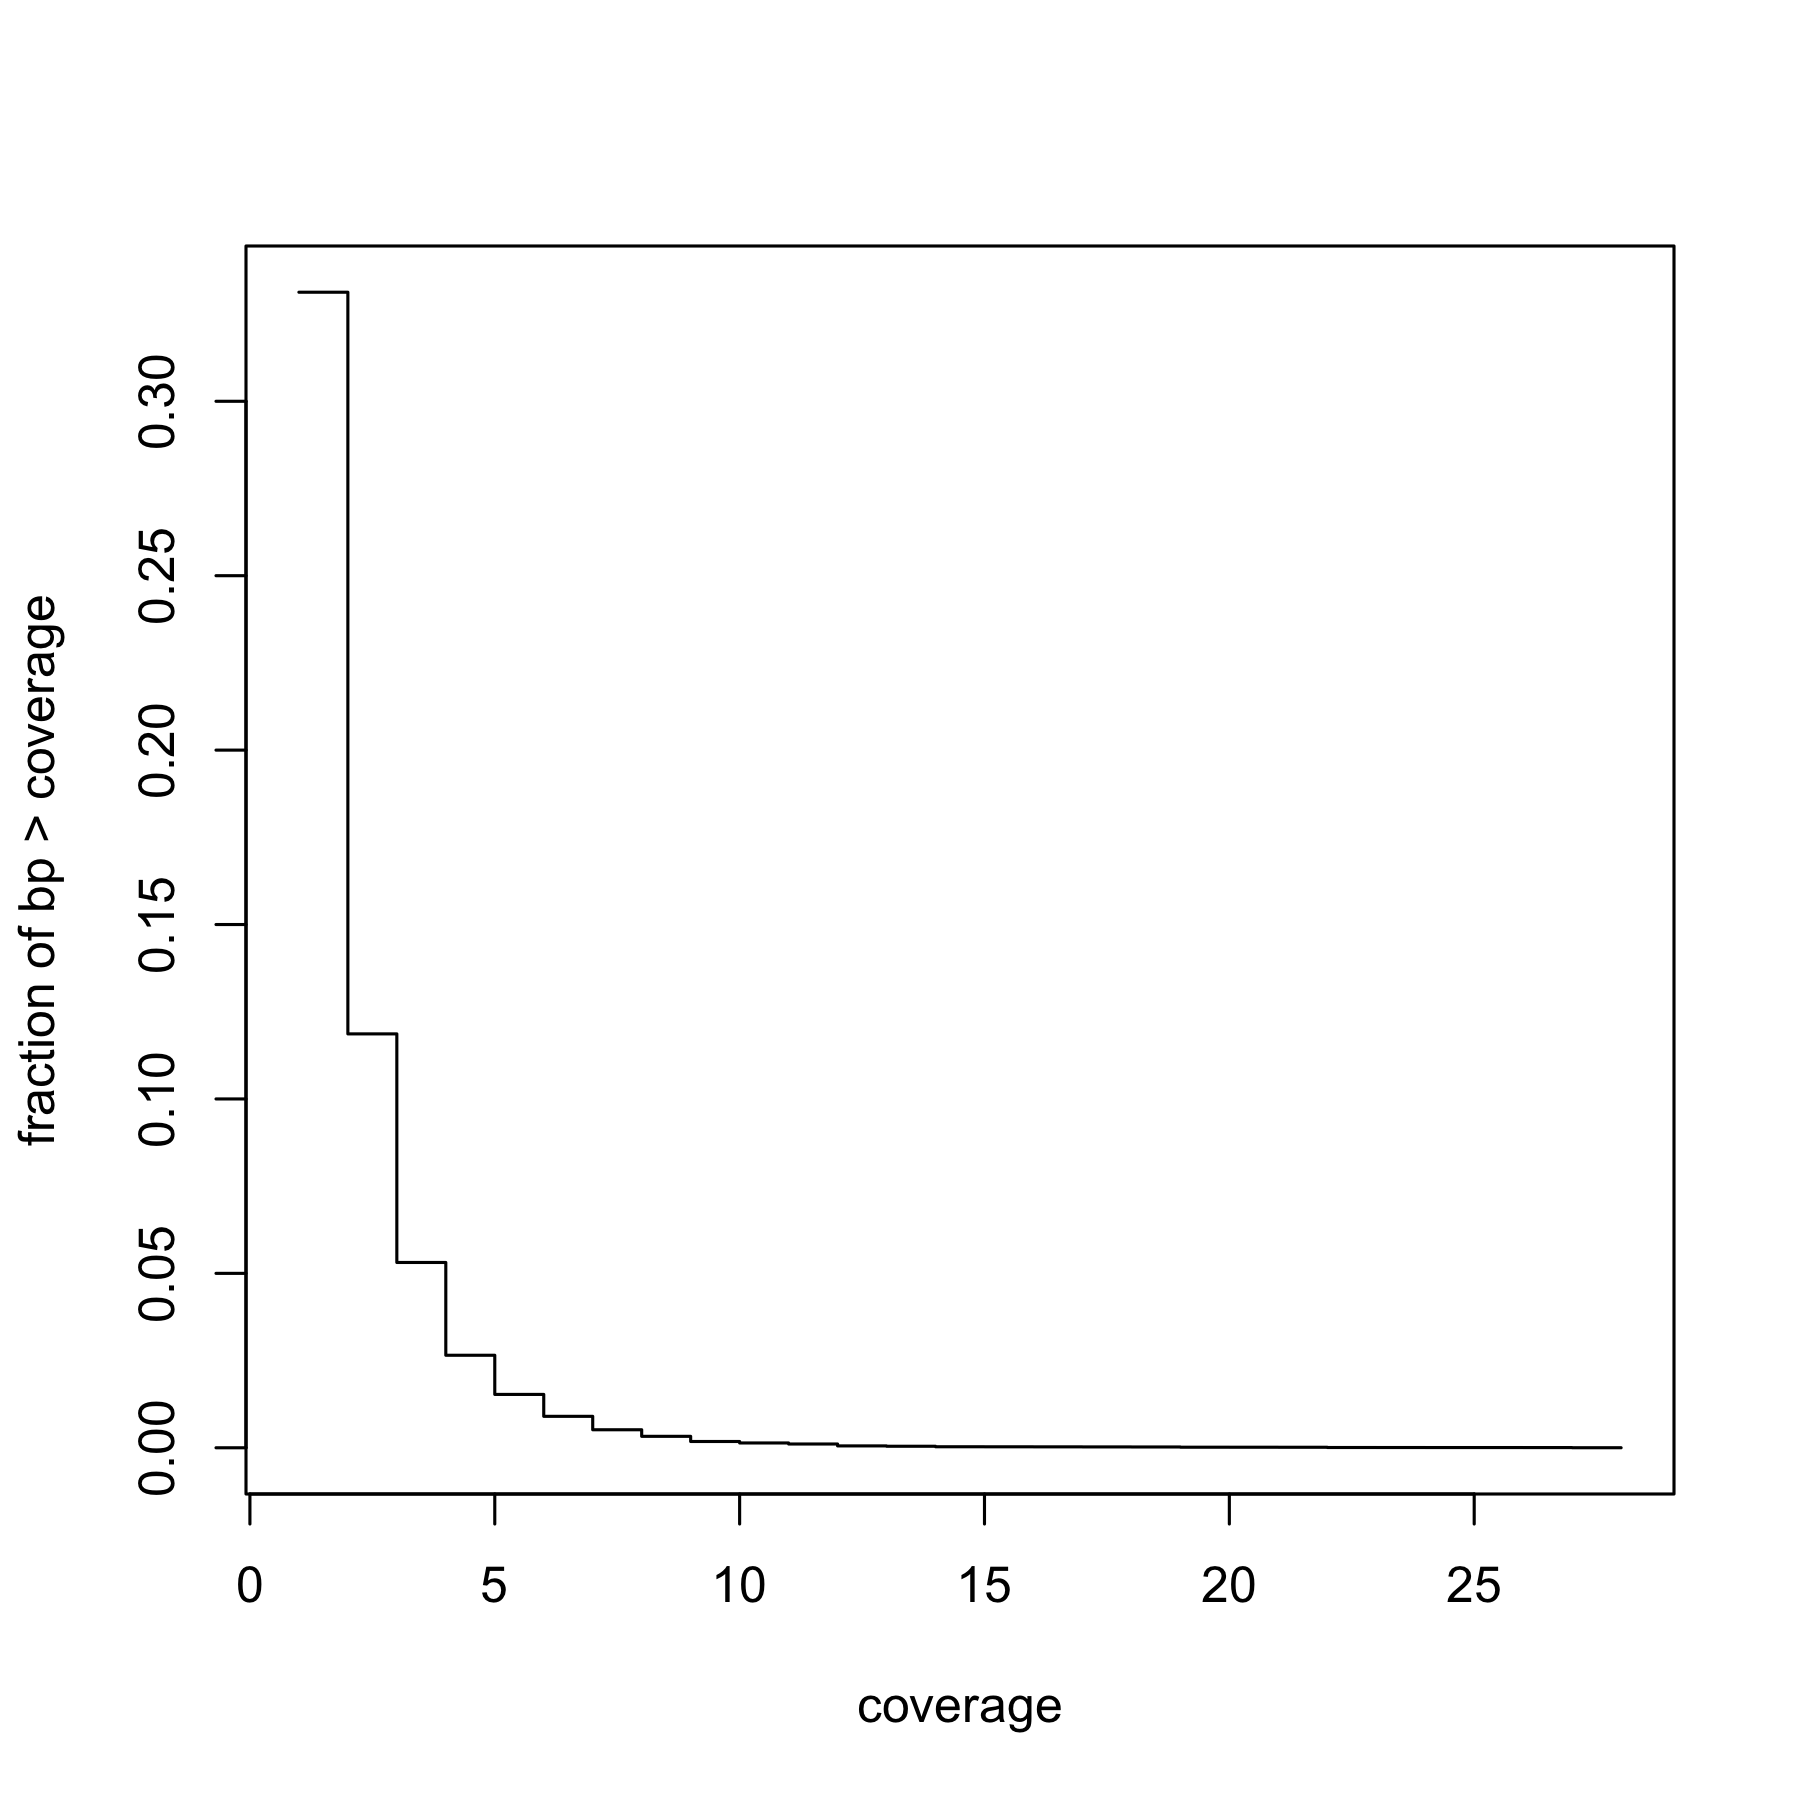
\includegraphics{tutorial-coalescence-plot}

\section{Jaccard Statistic}

In order to compare the DnaseI hypersenstivity across tissues, we will
employ the \software{bedtools jaccard} statistic, a measure of
similarity between two tracks. It is defined as the total width of
their intersection over the total width of their union.

We might expect, for example, that the similarity within a tissue is
higher than that between two tissues, and this is indeed the case:
\begin{Schunk}
\begin{Sinput}
> code <- bedtools_jaccard(
+     paste("-a fHeart-DS16621.hotspot.twopass.fdr0.05.merge.bed",
+           "-b fHeart-DS15839.hotspot.twopass.fdr0.05.merge.bed"))
> heart_heart <- eval(code)
> code <- bedtools_jaccard(
+     paste("-a fHeart-DS16621.hotspot.twopass.fdr0.05.merge.bed",
+           "-b fSkin_fibro_bicep_R-DS19745.hg19.hotspot.twopass.fdr0.05.merge.bed"))
> heart_skin <- eval(code)
> mstack(heart_heart=heart_heart, heart_skin=heart_skin)
\end{Sinput}
\begin{Soutput}
DataFrame with 2 rows and 5 columns
         name intersection     union   jaccard n_intersections
        <Rle>    <integer> <integer> <numeric>       <integer>
1 heart_heart     81269248 160493950 0.5063695          130852
2  heart_skin     28076951 164197278 0.1709952           73261
\end{Soutput}
\end{Schunk}
%
The generated code makes the statistic self-documenting:
\begin{Schunk}
\begin{Sinput}
> code
\end{Sinput}
\begin{Soutput}
{
    genome <- NA_character_
    gr_a <- import("fHeart-DS16621.hotspot.twopass.fdr0.05.merge.bed", 
        genome = genome)
    gr_b <- import("fSkin_fibro_bicep_R-DS19745.hg19.hotspot.twopass.fdr0.05.merge.bed", 
        genome = genome)
    intersects <- intersect(gr_a, gr_b, ignore.strand = TRUE)
    intersection <- sum(width(intersects))
    union <- sum(width(union(gr_a, gr_b, ignore.strand = TRUE)))
    ans <- DataFrame(intersection, union, jaccard = intersection/union, 
        n_intersections = length(intersects))
    ans
}
\end{Soutput}
\end{Schunk}

We can compute the statistic over all pairs of samples using
functionality included with R, through the \Rpackage{parallel}
package. There is no need to learn yet another syntax, such as that of
the \software{parallel} UNIX utility. Nor do we need to download a
custom python script, and repeatedly call perl and awk.
\begin{Schunk}
\begin{Sinput}
> files <- Sys.glob("*.merge.bed")
> names(files) <- sub("\\..*", "", files)
> ans <- outer(files, files, 
+              function(a, b) mcmapply(do_bedtools_jaccard, a, b, 
+                                      mc.cores=4))
> jaccard <- apply(ans, 1:2, function(x) x[[1]]$jaccard)
\end{Sinput}
\end{Schunk}

Since we are already in R, it is easy to create a simple plot:
\begin{Schunk}
\begin{Sinput}
> palette <- colorRampPalette(c("lightblue", "darkblue"))(9)
> heatmap(jaccard, col=palette, margin=c(14, 14))
\end{Sinput}
\end{Schunk}
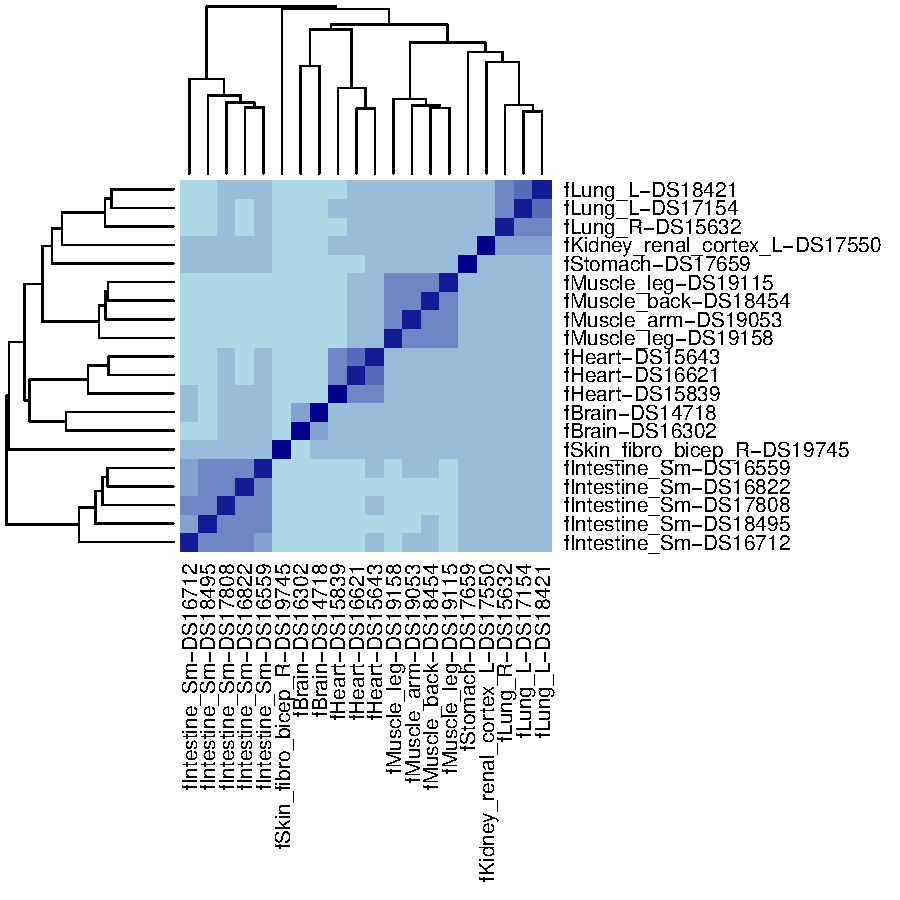
\includegraphics{tutorial-jaccard-plot}

\section{Exercises}

These were adapted from the \software{bedtools} tutorial. Try to
complete these exercises using \Bioconductor{} directly.

\begin{enumerate}
\item Create a \Rclass{GRanges} containing the non-exonic regions of
  the genome.
\item Compute the average distance from the GWAS SNPs to the closest
  exon (Hint: \Rcode{?bedtools\_closest} and
  \Rcode{?distanceToNearest}).
\item Compute the exon coverage in 500kb windows across the genome
  (Hint: \Rcode{?bedtools\_makewindows} and \Rcode{?tileGenome}).
\item How many exons are completely overlapped by an enhancer (from
  \file{hesc.chromHmm.bed}) (Hint: \Rcode{?`\%within\%`})?
\item What fraction of the disease-associated SNPs are exonic 
  (Hint: (Hint: \Rcode{?`\%over\%`}))?
\item Create intervals representing the canonical 2bp splice sites on
  either side of each exon (bonus: exclude splice sites at the first
  and last exons) (Hint: \Rcode{?bedtools\_flank},
  \Rcode{?intronsByTranscript}).
\item Which hESC ChromHMM state represents the most number of base
  pairs in the genome? (Hint: \Rcode{?xtabs}).
\end{enumerate}

\subsection{Answers}
Below, we give the \software{bedtools}-style answer first, followed by
the essential call against the \Bioconductor{} API.

First, we load the files into \R{} objects for convenience:
\begin{Schunk}
\begin{Sinput}
> genome <- import("hg19.genome")
> exons <- import("exons.bed", genome=genome)
> gwas <- import("gwas.bed", genome=genome)
> hesc.chromHmm <- import("hesc.chromHmm.bed", genome=genome)
\end{Sinput}
\end{Schunk}

Here are the numbered answers:

\begin{enumerate}
\item 
\begin{Schunk}
\begin{Sinput}
> bedtools_complement("-i exons.bed -g hg19.genome")
\end{Sinput}
\begin{Soutput}
{
    genome <- import("hg19.genome")
    gr_a <- import("exons.bed", genome = genome)
    ans <- setdiff(as(seqinfo(gr_a), "GRanges"), unstrand(gr_a))
    ans
}
\end{Soutput}
\begin{Sinput}
> ## or without HelloRanges:
> setdiff(as(seqinfo(exons), "GRanges"), unstrand(exons))
\end{Sinput}
\begin{Soutput}
GRanges object with 229334 ranges and 0 metadata columns:
           seqnames               ranges strand
              <Rle>            <IRanges>  <Rle>
       [1]     chr1       [    1, 11873]      *
       [2]     chr1       [12228, 12612]      *
       [3]     chr1       [12722, 13220]      *
       [4]     chr1       [14830, 14969]      *
       [5]     chr1       [15039, 15795]      *
       ...      ...                  ...    ...
  [229330]     chrY [59337237, 59337948]      *
  [229331]     chrY [59338151, 59338753]      *
  [229332]     chrY [59338860, 59340193]      *
  [229333]     chrY [59340279, 59342486]      *
  [229334]     chrY [59343489, 59373566]      *
  -------
  seqinfo: 93 sequences from hg19 genome
\end{Soutput}
\end{Schunk}
\item 
\begin{Schunk}
\begin{Sinput}
> bedtools_closest("-a gwas.bed -b exons.bed -d")
\end{Sinput}
\begin{Soutput}
{
    genome <- Seqinfo(genome = NA_character_)
    gr_a <- import("gwas.bed", genome = genome)
    gr_b <- import("exons.bed", genome = genome)
    hits <- nearest(gr_a, gr_b, ignore.strand = TRUE, select = "all")
    ans <- pair(gr_a, gr_b, hits, all.x = TRUE)
    mcols(ans)$distance <- distance(ans)
    ans
}
\end{Soutput}
\begin{Sinput}
> ## or 
> distanceToNearest(gwas, exons)
\end{Sinput}
\begin{Soutput}
Hits object with 17674 hits and 1 metadata column:
          queryHits subjectHits |  distance
          <integer>   <integer> | <integer>
      [1]         1         235 |      1319
      [2]         2         249 |         0
      [3]         3         426 |         0
      [4]         4        1160 |      2385
      [5]         5        1160 |      2894
      ...       ...         ... .       ...
  [17670]     17676      455396 |       371
  [17671]     17677      455396 |       371
  [17672]     17678      455464 |      5898
  [17673]     17679      455674 |    324706
  [17674]     17680      456097 |    135628
  -------
  queryLength: 17680 / subjectLength: 459752
\end{Soutput}
\end{Schunk}
\item
\begin{Schunk}
\begin{Sinput}
> code <- bedtools_makewindows("-g hg19.genome -w 500000")
> code
\end{Sinput}
\begin{Soutput}
{
    genome <- import("hg19.genome")
    ans <- tile(as(genome, "GRanges"), width = 500000L)
    ans
}
\end{Soutput}
\begin{Sinput}
> windows <- unlist(eval(code))
> R_bedtools_intersect(windows, exons, c=TRUE)
\end{Sinput}
\begin{Soutput}
{
    genome <- Seqinfo(genome = NA_character_)
    gr_a <- windows
    gr_b <- exons
    ans <- gr_a
    mcols(ans)$overlap_count <- countOverlaps(gr_a, gr_b, ignore.strand = TRUE)
    ans
}
\end{Soutput}
\begin{Sinput}
> ## or
> str(countOverlaps(tileGenome(seqinfo(exons), tilewidth=500000), 
+                   exons))
\end{Sinput}
\begin{Soutput}
 int [1:6275] 37 197 477 445 209 96 83 271 9 12 ...
\end{Soutput}
\end{Schunk}
\item 
\begin{Schunk}
\begin{Sinput}
> bedtools_intersect(
+     paste("-a exons.bed -b <\"grep Enhancer hesc.chromHmm.bed\"",
+           "-f 1.0 -wa -u"))
\end{Sinput}
\begin{Soutput}
{
    genome <- Seqinfo(genome = NA_character_)
    gr_a <- import("exons.bed", genome = genome)
    gr_b <- import(BEDFile(pipe("grep Enhancer hesc.chromHmm.bed")), 
        genome = genome)
    hits <- findOverlaps(gr_a, gr_b, ignore.strand = TRUE, type = "within")
    gr_a[countQueryHits(hits) > 0L]
}
\end{Soutput}
\begin{Sinput}
> quote(length(ans))
\end{Sinput}
\begin{Soutput}
length(ans)
\end{Soutput}
\begin{Sinput}
> ## or
> sum(exons %within% 
+     subset(hesc.chromHmm, grepl("Enhancer", name)))
\end{Sinput}
\begin{Soutput}
[1] 13746
\end{Soutput}
\end{Schunk}
\item 
\begin{Schunk}
\begin{Sinput}
> bedtools_intersect("-a gwas.bed -b exons.bed -u")
\end{Sinput}
\begin{Soutput}
{
    genome <- Seqinfo(genome = NA_character_)
    gr_a <- import("gwas.bed", genome = genome)
    gr_b <- import("exons.bed", genome = genome)
    subsetByOverlaps(gr_a, gr_b, ignore.strand = TRUE)
}
\end{Soutput}
\begin{Sinput}
> quote(length(gr_a)/length(ans))
\end{Sinput}
\begin{Soutput}
length(gr_a)/length(ans)
\end{Soutput}
\begin{Sinput}
> ## or
> mean(gwas %over% exons)
\end{Sinput}
\begin{Soutput}
[1] 0.09162896
\end{Soutput}
\end{Schunk}
\item 
\begin{Schunk}
\begin{Sinput}
> bedtools_flank("-l 2 -r 2 -i exons.bed -g genome.txt")
\end{Sinput}
\begin{Soutput}
{
    genome <- Seqinfo(genome = "genome.txt")
    gr_a <- import("exons.bed", genome = genome)
    left <- flank(gr_a, 2, ignore.strand = TRUE)
    right <- flank(gr_a, 2, start = FALSE, ignore.strand = TRUE)
    ans <- zipup(Pairs(left, right))
    ans
}
\end{Soutput}
\begin{Sinput}
> ## or, bonus:
> exons <- keepStandardChromosomes(exons)
> txid <- sub("_exon.*", "", exons$name)
> tx <- split(exons, txid)
> bounds <- range(tx)
> transpliced <- lengths(bounds) > 1
> introns <- unlist(psetdiff(unlist(bounds[!transpliced]), 
+                            tx[!transpliced]))
> Pairs(resize(introns, 2L), resize(introns, 2L, fix="end"))
\end{Sinput}
\begin{Soutput}
Pairs object with 389830 pairs and 0 metadata columns:
                                first                     second
                            <GRanges>                  <GRanges>
       [1]    chr12:9220777-9220778:-    chr12:9220436-9220437:-
       [2]    chr12:9221334-9221335:-    chr12:9220821-9220822:-
       [3]    chr12:9222339-9222340:-    chr12:9221439-9221440:-
       [4]    chr12:9223082-9223083:-    chr12:9222410-9222411:-
       [5]    chr12:9224953-9224954:-    chr12:9223175-9223176:-
       ...                        ...                        ...
  [389826] chr9:123626325-123626326:- chr9:123625028-123625029:-
  [389827] chr9:123627986-123627987:- chr9:123626395-123626396:-
  [389828] chr9:123628304-123628305:- chr9:123628109-123628110:-
  [389829] chr9:123629146-123629147:- chr9:123628375-123628376:-
  [389830] chr9:123631084-123631085:- chr9:123629244-123629245:-
\end{Soutput}
\begin{Sinput}
> ## better way to get introns:
> library(TxDb.Hsapiens.UCSC.hg19.knownGene)
> txdb <- TxDb.Hsapiens.UCSC.hg19.knownGene
> introns <- unlist(intronsByTranscript(txdb))
\end{Sinput}
\end{Schunk}
\item
\begin{Schunk}
\begin{Sinput}
> system.time(names(which.max(xtabs(width ~ name, 
+                                   hesc.chromHmm))))
\end{Sinput}
\begin{Soutput}
   user  system elapsed 
  0.080   0.019   0.097 
\end{Soutput}
\begin{Sinput}
> ## or
> names(which.max(sum(with(hesc.chromHmm, 
+                          splitAsList(width, name)))))
\end{Sinput}
\begin{Soutput}
[1] "13_Heterochrom/lo"
\end{Soutput}
\begin{Sinput}
> ## or
> df <- aggregate(hesc.chromHmm, ~ name, totalWidth=sum(width))
> df$name[which.max(df$totalWidth)]
\end{Sinput}
\begin{Soutput}
[1] 13_Heterochrom/lo
15 Levels: 10_Txn_Elongation 11_Weak_Txn ... 9_Txn_Transition
\end{Soutput}
\end{Schunk}
\end{enumerate}


\bibliography{tutorial}

\end{document}
